\chapter{Auto-riferimento} \label{ch:capitolo6}
\section{Autoriferimento}
\subsection{Teorema di ricursione di Turing}
\textbf{Teorema}\\
Sia $f: N $ x $N \mapsto N$ una funzione calcolabile (parziale). Esiste effettivamente $z \in N$ tale che:
\begin{center}
    $\phi_z (y) = f(z,y).$
\end{center}
\textbf{Osservazione}
\begin{itemize}
    \item Il programma di una macchina di Turing può accedere al suo codice
    
    \item Si può calcolare una funzione che dipende anche dalla macchina che la calcola
\end{itemize}
\textbf{Esempio}\\
Cosa calcola la seguente macchina di Turing?.\\
Su input x
\begin{figure}[htp]
    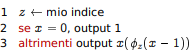
\includegraphics[scale=0.8]{tesi_stile/img/cap6f1.png}
\end{figure}
\subsection{Teorema s-m-n}
\textbf{Teorema}\\
Sia $f : N $ x $N \mapsto N$ una funzione (parziale) calcolabile. Allora esiste una funzione calcolabile totale $t:N \mapsto N$ tale che
\begin{center}
    $\phi_{t(x)} (y)=f(x,y)$ con $x,y \in N.$
\end{center}
\textbf{Osservazione}\\
Questo teorema ci dice che ogni funzione di due variabili f(x,y) si può calcolare nel modo seguente:
\begin{itemize}
    \item costruisco una macchina di Turing $M = M_t(x)$ che dipende solo da x
    
    \item eseguo M sull'input y
\end{itemize}
\newpage
\subsection{Dimostrazione del Teorema s-m-n}
\textbf{Dimostrazione}\\
Per ogni $x \in N,$ sia $g_x: N \mapsto N$ la funzione definita da $g_x(y) = f(x,y)$.\\\\
Una macchina di Turing per calcolare gx si ottiene concatenando
\begin{itemize}
    \item le istruzioni per stampare x sul nastro prima di y
    
    \item le istruzioni della macchina di Turing che calcola f .
\end{itemize}
Dato x, si può effettivamente costruire tale macchina e calcolarne l’indice.\\
Se t è la funzione che esegue questo calcolo, si avrà\\
\begin{center}
    $f(x,y)=g_x(y) = \phi_{t(x)}(y).$\\
\end{center}
\begin{figure}[htp]
    \centering
    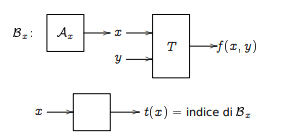
\includegraphics[scale=0.8]{tesi_stile/img/cap6foto2.png}
\end{figure}
\newpage
\subsection{Dimostrazione del Teorema di Ricursione}
Per ogni $x \in N$, sia $g_x : N \mapsto N$ la funzione definita da $g_x(y) = f(x,y)$.
\begin{figure}[htp]
    \centering
    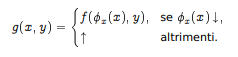
\includegraphics[scale=0.9]{tesi_stile/img/cap6f3.png}
\end{figure}
\\Una macchina di Turing per calcolare $g_x$ si ottiene concatenando.\\
Per il Teorema s-m-n, c’è una funzione totale t = $\phi_v$ tale che\\
\begin{center}
    $\phi_{t(z)}(y) = g(x,y)$ con $x,y \in N$
\end{center}
Posto $z = t(v) = \phi_v (v)$, si ha
\begin{center}
   $ \phi_z(y) = \phi_t{(v)}(y) = g(v,y)=f(\phi_v(v), y) = f (z,y)$
\end{center}
\newpage
\subsection{Costruzione}
\begin{figure}[htp]
    \centering
    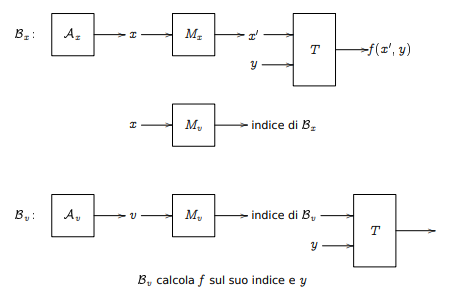
\includegraphics[scale=1]{tesi_stile/img/cap6f4.png}
\end{figure}
\newpage
\subsection{Esempio}
È indecidibile se una macchina di Turing accetta 1.\\
Se così non fosse, potremmo costruire una macchina di Turing con il seguente programma\\
Su input x.\\
\begin{figure}[htp]
    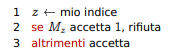
\includegraphics[scale=0.8]{tesi_stile/img/cap6f5.png}
\end{figure}\\
\begin{center}
    \textbf{Contraddizione!}
\end{center}
Nuova dimostrazione dell’indecidibilità del problema dell’arresto:\\
Se fosse decidibile, potremmo costruire una macchina di Turing con il seguente programma.\\
Su input x.\\
\begin{figure}[htp]
    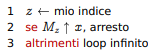
\includegraphics[scale=0.8]{tesi_stile/img/cap6f6.png}
\end{figure}\\
\begin{center}
    \textbf{Contraddizione!}
\end{center}
\newpage
\subsection{Teorema del punto fisso}
\textbf{Teorema}\\
 Sia $t : N \mapsto N$ una funzione calcolabile totale.\\
 Esiste effettivamente $z \in N$ tale che\\
 \begin{center}
     $\phi_z = \phi_t(z)$
 \end{center}
 \textbf{Dimostrazione}\\
La funzione $f : N$ x $N \mapsto N$ definita da $f(x,y) = \phi_{t(x)}(y)$ con $x,y \in N$, è
calcolabile. Per il Teorema di Recursione ci sarà $z \in N$ tale che\\
\begin{center}
    $\phi_z (y) = f (z,y) = \phi_t(z) (y),  y \in N.$
\end{center}
\textbf{Oppure}\\
Basta considerare la funzione calcolata dalla procedura.\\
Su input x\\
\begin{figure}[htp]
    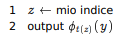
\includegraphics[scale=0.8]{tesi_stile/img/cap6f7.png}
\end{figure}
\newpage
\subsection{Teorema di Radice}
\textbf{Teorema}\\
Sia P una famiglia di funzioni calcolabili. L’insieme.\\
\begin{center}
    $R = \{x \in N | \phi_x \in P\}$
\end{center}
è indecidibile, purchè $R\neq \varnothing$, $N$.\\\\
\textbf{Dimostrazione}\\
Per assurdo, supponiamo che R sia decidibile e $R \neq \varnothing$, $N$. 
\begin{itemize}
    \item Possiamo trovare $i \in R$ e $j \notin R$.
    
    \item Definiamo la funzione $f : N $ x $N \mapsto N$ con
\end{itemize}
\begin{figure}[htp]
    \centering
    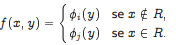
\includegraphics[scale=0.8]{tesi_stile/img/cap6f8.png}
\end{figure}
Per il Teorema di Recursione ci sarà $z \in N$ tale che $\phi_z (y) = f(z,y)$.\\
Ma allora se $z \notin R$, si ha $\phi_z = \phi_i \in R$, mentre se $z \in R$, si ha $\phi_z = \phi_j \notin R$.\\
\begin{center}
    \centering
    \textbf{Contraddizione!}.
\end{center}
\newpage
\subsection{Macchina di Turing minimali}
\textbf{Definizione}\\
Una macchina di Turing è minimale se non esistono macchine di Turing con un minor numero di stati che calcolano la stessa funzione.\\\\
\textbf{Osservazione}\\
Legata alle nozioni di complessità di Kolmogorov, entropia, compressibilità.\\\\
\textbf{Proposizione}\\
È indecidibile se una macchina di Turing è minimale.\\\\
\textbf{Dimostrazione}\\
Se così non fosse, avremmo una macchina di Turing che:\\
Su input x
\begin{figure}[htp]
    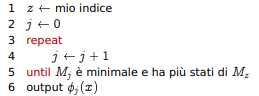
\includegraphics[scale=0.8]{tesi_stile/img/cap6f9.png}
\end{figure}
\\Ma allora Mz è equivalente a una macchina minimale con più stati: \textbf{assurdo}